\documentclass{article}
\usepackage{graphicx} % Required for inserting images
\usepackage{amsmath}
\usepackage{amssymb}
\usepackage{comment}
\usepackage{minted}

\title{Oblig STK4021}
\author{Daniel Steeneveldt}
\date{October 2024}

\begin{document}

\maketitle
\section{Problem 1}
Let $y$ be a Bernoulli random variable with parameter $\theta \in (0,1)$, so $y$ has the mass function $f_\theta(y) = \theta^y(1-\theta)^{1-y}$, for $y = 0,1$.
\begin{enumerate}

    \item[(a)] Find the mean and variance of $y$, as functions of $\theta$.
    

    %solution

    \textbf{Sol:}
    \par
    The mean of $y$ is given by

    \[
    \mathbb{E}(y) = \sum y f_{\theta} (y) = 0 \cdot (1-\theta) + 1 \cdot \theta = \theta
    \]

    The variance is given by
    \begin{align*}
    \text{Var}(y) &= \mathbb{E}(y^2) - \mathbb{E}(y)^2 \\
    &= \sum y^2 f_{\theta} (y) - \theta^2 \\
    &= 0^2 \cdot (1-\theta) + 1^2 \cdot \theta - \theta^2 \\
    &= \theta - \theta^2 \\
    &= \theta(1- \theta)
    \end{align*}



    We want to estimate $\theta$ using the loss function $L(t, \theta) = \frac{(t-\theta)^2}{\theta(1-\theta)}$.
    
    \item[(b)] Verify that the maximum likelihood estimator for $\theta$ is $y$ itself, and that this estimator has unit (frequentist) risk. That is, show that $R(y, \theta) = 1$.

    \textbf{Sol:}
    \par
    The maximum likelihood estimator for one sample is just the pdf evaulated at $y$
    \[
    \mathcal{L} = f_{\theta}(y) = \theta^y (1-\theta)^{1-y}
    \]
    log-likelihood
    \[
    \ell = y \log(\theta) + (1-y) \log(1-\theta)
    \]
    Finding minima
    \[
        0 = \frac{\partial \ell}{\partial \theta} = \frac{y}{\theta} - \frac{1-y}{1-\theta} 
    \]
    \begin{align*}
        \frac{y}{1-y} =& \frac{\theta}{1-\theta}\\
        y =& \theta
    \end{align*}

    Now introduce the Bayesian machinery. Let $\theta \sim \text{Beta}(a,b)$ in the prior distribution, where $a, b > 0$. That is, $\theta$ has prior density
    \[
    \pi(\theta) = \frac{\Gamma(a+b)}{\Gamma(a)\Gamma(b)} \theta^{a-1}(1-\theta)^{b-1}, \quad 0 < \theta < 1.
    \]
    
    \item[(c)] Show that $\mathbb{E}[\theta] = \frac{a}{a+b}$ and
    \[
    \mathbb{E}\left[\frac{1}{\theta}\right] = 
    \begin{cases} 
    \frac{(a+b-1)}{(a-1)} & \text{if } a > 1 \\
    \infty & \text{otherwise.}
    \end{cases}
    \]

    \textbf{Solution:}
    \par

    \begin{align*}
    \mathbb{E}(\theta) =& \int_{-\infty}^{\infty} \theta \pi(\theta) d \theta\\
                        =& \int_0^1 \theta \frac{\Gamma(a + b)}{\Gamma(a)  \Gamma(b)} \theta^{a-1} (1 - \theta)^{b-1} d \theta\\
                        =& \frac{\Gamma(a + b)}{\Gamma(a)   \Gamma(b)} \int_0^1 \theta^{a}(1-\theta)^{b-1} d \theta\\
                        =&  \frac{\Gamma(a + b)}{\Gamma(a)   \Gamma(b)} \left(  \frac{\Gamma(a +1  + b)}{\Gamma(a + 1) \Gamma(b)}\right)^{-1}\\
                        =& \frac{\Gamma(a + b)}{\Gamma(a)  \Gamma(b)} \frac{a\Gamma(a) \Gamma(b)}{(a+b) \Gamma(a+b)}\\
                        =& \frac{a}{a+b}
    \end{align*}

    \begin{align*}
        \mathbb{E}\left(\frac{1}{\theta}\right) =& \int_{-\infty}^{\infty} \frac{1}{\theta} \pi(\theta) d \theta\\
                    =& \int_0^1 \frac{1}{\theta} \frac{\Gamma(a + b)}{\Gamma(a)  \Gamma(b)} \theta^{a-1} \theta{b-1} d \theta\\
                    =& \frac{\Gamma(a + b)}{\Gamma(a) \Gamma(b)} \int_0^1 \theta^{a-2}(1-\theta)^{b-1} d \theta\\
                    =& \frac{\Gamma(a + b)}{\Gamma(a) \Gamma(b)} \int_0^1 \theta^{(a-1)-1}(1-\theta)^{b-1} d \theta
    \end{align*}

    The integral we recognize again as an integral of a beta distribution with coefficients $a-1$ and $b$. The distribution is only defined for coefficients greater than 0, thus $a > 1$. We can also show this by considering the integral near 0.
    
    \begin{align*}
        \int_0^1 \theta^{(a-1)-1}(1-\theta)^{b-1} d \theta \geq& \int_0^{\epsilon} \theta^{(a-1)-1}(1-\theta)^{b-1} d \theta\\
         \geq&  \frac{1}{2^{b-1}} \int_0^{\epsilon} \theta^{(a-1)-1} d \theta
    \end{align*}
    The integral is only finite if the exponent is greater than $-1$ i.e $a > 1$.
    \par
    Continuing $\mathbb{E}\left(\frac{1}{\theta}\right)$, for $a > 1$
    \begin{align*}
        \mathbb{E}\left(\frac{1}{\theta}\right) =& \\
                    =&  \frac{\Gamma(a + b)}{\Gamma(a) \Gamma(b)} \left(  \frac{\Gamma(a -1 + b)}{\Gamma(a - 1)   \Gamma(b)}\right)^{-1}\\
                    =& \frac{\Gamma(a + b)}{\Gamma(a) \Gamma(b)} \frac{(a-1)\Gamma(a)  \Gamma(b)}{(a+b-1) \Gamma(a+b)}\\
                    =& \frac{(a+b-1)}{(a-1)}
    \end{align*}

    \item[(d)] Find the distribution of $\gamma = 1-\theta$.
    
    \textbf{Solution:}
    \par

    Here we need to use the change of variables formula. For $g$, we have that for $Y = g(X)$ the density of $Y$ is given by
    
    \[
    f_Y(y) = f_X(g^{-1}(y)) \left| \frac{d g^{-1}(y)}{dy} \right|
    \]
    For our case we have that $g(\theta) = 1-\theta$ and $g^{-1}(\gamma) = 1-\gamma$. The density of $\gamma$ is then given by

    \begin{align*}
    \pi_{\gamma}(\gamma) &= \pi(1-\gamma) \left| \frac{d(1-\gamma)}{d\gamma} \right|\\
     &= \pi(1-\gamma) \\
     &= \frac{\Gamma(a+b)}{\Gamma(a)  \Gamma(b)} (1-\gamma)^{a-1} \gamma^{b-1}\\
     &= \frac{\Gamma(a+b)}{\Gamma(a)  \Gamma(b)}  \gamma^{b-1}(1-\gamma)^{a-1}
    \end{align*}

    Which we recognize as Beta(b,a)
   


    
    \item[(e)] Show that $\pi(\theta)$ is a conjugate prior, and find the posterior distribution $\pi(\theta | y)$.
    
    \textbf{Solution:}
    \par
    We recognize that the Bernoulli and the Beta distrobution have the same form - jippie! We can ignore the normalizing $\pi(y)$ which is constant in $\theta$, and just look at the part of the likelihood times prior which is proportional to $\theta$.
    \begin{align*}
        \pi(\theta | y) &\propto f_{\theta}(y) \pi(\theta)\\
        &\propto \theta^y(1-\theta)^{1-y} \theta^{a-1}(1-\theta)^{b-1}\\
        &\propto \theta^{y+a-1}(1-\theta)^{1-y+b-1}
    \end{align*}
    Which we recognize as the functional form of a Beta distribution with parameters $y+a$ and $1-y+b$. Thus this is the posterior distribution.

    \item[(f)] From now on, assume that $a, b > 1$. Show that the Bayes estimator is given by
    \[\hat{\theta} = \frac{a + y - 1}{a + b - 1}.\]

    \textbf{Solution:}
    \par
    The Bayes estimator is the of the expected loss over the posterior distribution. The expected loss is given by  
    
    \begin{align*}
        \int_{\Theta} L(\theta, t) \pi(\theta | y) d\theta &= \int_{0}^{1} \frac{(t - \theta)^2}{\theta(1-\theta)} \pi(\theta | y) d\theta\\
    \end{align*}

    We want to minimize this, so we can differentiate and set to zero
    
    \begin{align*}
        0 &= \frac{\partial}{\partial t} \int_{0}^{1} \frac{(t - \theta)^2}{\theta(1-\theta)} \pi(\theta | y) d\theta\\
        &= \int_{0}^{1} \frac{2(t - \theta)}{\theta(1-\theta)} \pi(\theta | y) d\theta\\
        &\propto \int_{0}^{1} \frac{(t - \theta)}{\theta(1-\theta)} \theta^{a'-1} \left(1 - \theta \right)^{b'- 1} d\theta\\
        t \int_0^1 \theta ^ {a'-1-1} (1-\theta)^{b'-1-1} d\theta &= \int_0^1 \theta^{a'-1} (1-\theta)^{b'-1-1} d\theta\\
        t \frac{\Gamma(a'-1) \Gamma(b'-1)}{\Gamma(a'+b'-2)} &= \frac{\Gamma(a') \Gamma(b'-1)}{\Gamma(a'+b'-1)}\\
        t \frac{\Gamma(a'-1)}{\Gamma(a'+b'-2)} &= \frac{ (a - 1) \Gamma(a' - 1)}{ (a' + b - 2) \Gamma(a'+b'-2)}\\
        t &= \frac{a'- 1}{a' + b' - 1}\\
        t &= \frac{a + y - 1}{a + b - 1}
    \end{align*}

    This is our Bayes estimator $\hat \theta$


    
    
    \item[(g)] \textbf{Show that the minimal Bayes risk is}
    \[\frac{1}{a + b - 1}.\]
    
    \textbf{Solution:}
    \par
    The minimal bayes risk is given by 
    \begin{align*}
        \int_{0}^{1} L(\theta, \hat{\theta}) \pi(\theta | y) d\theta &= \int_{0}^{1} \frac{(\hat{\theta} - \theta)^2}{\theta(1-\theta)} \pi(\theta | y) d\theta\\
        &= \int_{0}^{1} \frac{\left(\hat{\theta}^2 -2\hat{\theta} \theta + \theta^2 \right)}{\theta(1-\theta)} \pi(\theta | y) d\theta\\
        &= \hat{\theta}^2 \int_0^1 \frac{1}{\theta(1-\theta)} \pi(\theta | y) d\theta - 2\hat{\theta} \int_0^1 \frac{1}{1-\theta}\pi(\theta | y) d\theta + \int_0^1 \frac{\theta}{(1-\theta)} \pi(\theta | y) d\theta\\
        &= \hat{\theta}^2 A -2 \hat{\theta} B + C       
    \end{align*}
Calling the normalizing constant $c_{\pi | y} = \frac{\Gamma(a+b+1)}{\Gamma(a+y) \Gamma(b-y+1)}$ , we can write $A$ as

\begin{align*}
    A =  \int_0^1 \frac{1}{\theta(1-\theta)} \pi(\theta | y) d\theta &=  c_{\pi | y} \int_0^1 \frac{1}{\theta(1-\theta)} \theta^{a + y -1} (1-\theta)^{b-y} d\theta\\
    &=  c_{\pi | y} \int_0^1 \theta^{a+y-1-1} (1-\theta)^{b-y-1} d\theta\\
    &=  c_{\pi | y} \frac{\Gamma(a+y-1) \Gamma(b-y)}{\Gamma(a+b-1)}\\
    &=  \frac{\Gamma(a+b+1)}{\Gamma(a+y) \Gamma(b-y+1)} \frac{\Gamma(a+y-1) \Gamma(b-y)}{\Gamma(a+b-1)}\\
    &= \frac{(a+b)(a+b-1)}{(a+y-1)(b-y)}\\
\end{align*}

$B$ is given by

\begin{align*}
    B &= \int_0^1 \frac{1}{1-\theta} \pi(\theta | y) d\theta\\
    &= \int_1^0 \frac{1}{\gamma} \pi(1-\gamma | y) (-d\gamma), \quad \gamma = 1-\theta\\
    &= \int_0^1 \frac{1}{\gamma} \pi(1-\gamma | y) d\gamma, \quad \text{this var change switches a and b}\\
    &= \frac{b'+a'-1}{b'-1}, \quad \text{from c)}, a' = a + y, b' = b - y + 1 \\
    &= \frac{a+b}{b-y}
\end{align*}

$C$ is given by

\begin{align*}
    C &= \int_0^1 \frac{\theta}{1-\theta} \pi(\theta | y) d\theta\\
\end{align*}
Using that
$\frac{\theta}{1-\theta} = \frac{1}{1-\theta} - 1$
And the same change of variables as in $B$ with the result c) we get

\begin{align*}
    C &= \int_0^1 \frac{1}{1-\theta} \pi(\theta | y) d\theta - 1\\
    &= \frac{a+b}{b-y} - 1\\
    &= \frac{a+y}{b-y}\\
\end{align*}


The minimal Bayes risk is then

\begin{align*}
    BR^* &= \hat{\theta}^2 A -2 \hat{\theta} B + C\\
    &= \left(\frac{a + y - 1}{a + b - 1}\right)^2 \frac{(a+b)(a+b-1)}{(a+y-1)(b-y)} -2 \frac{a + y - 1}{a + b - 1} \frac{a+b}{b-y} + \frac{a+y}{b-y}\\
    &= -\frac{(a + y - 1)(a+b)}{(a + b - 1)(b-y)} + \frac{a+y}{b-y}\\
    &= \frac{(a + y - 1)(a + b)}{(a + b - 1)(b - y)} \cdot \frac{-a - b + y + 1}{a + b - 1} + \frac{a + y}{b - y} \\
    &= \frac{-(a + y - 1)(a + b)}{(a + b - 1)(b - y)} + \frac{a + y}{b - y} \\
    &= \frac{-(a + y - 1)(a + b) + (a + y)(a + b - 1)}{(a + b - 1)(b - y)} \\
    &= \frac{-a(a + b) - y(a + b) + a(a + b - 1) + y(a + b - 1)}{(a + b - 1)(b - y)} \\
    &= \frac{-a(a + b) - y(a + b) + a(a + b) - a + y(a + b) - y}{(a + b - 1)(b - y)} \\
    &= \frac{-a - y + a + b}{(a + b - 1)(b - y)} \\
    &= \frac{b - y}{(a + b - 1)(b - y)} \\
    &= \frac{1}{a + b - 1}
\end{align*}



\end{enumerate}

\section{Problem 2}


\begin{equation}
    \label{eq:trajectory}
    \gamma(t) = \left( \begin{array}{c} 
    v_0 \cos(\theta) t \\ 
    v_0 \sin(\theta) t - \frac{1}{2} g t^2 
    \end{array} \right),
\end{equation}

\begin{enumerate}
    \item[(a)] Show that if an arrow follows the parameterization \ref{eq:trajectory}, then it will travel a distance 
    \item[] $x = v_0^2 \sin(2\theta)/g$ before it lands.


\textbf{Solution:}
\par
The arrow hits the ground when $y=0$

\begin{align*}
    v_0 \sin(\theta) t - \frac{1}{2} g t^2 &= 0\\
    t(v_0 \sin(\theta) - \frac{1}{2} g t) &= 0
\end{align*}

\[
    t = 0 \quad \text{or} \quad v_0 \sin(\theta) = \frac{1}{2} g t \quad \Rightarrow t = \frac{2v_0 \sin(\theta)}{g}
\]

$t=0$ is just the starting point. The distance traveled is then



\begin{align*}
    x &= v_0 \cos(\theta) t\\
    &= v_0 \cos(\theta) \frac{2v_0 \sin(\theta)}{g}\\
    &= \frac{2v_0^2 \sin(\theta) \cos(\theta)}{g}\\
    &= \frac{v_0^2 \sin(2\theta)}{g}
\end{align*}



\begin{table}[h!]
    \centering
    \begin{tabular}{|c|c|c|c|c|c|}
    \hline
    43.50 & 41.50 & 43.00 & 41.82 & 44.55 \\
    42.86 & 41.77 & 43.22 & 41.63 & 44.02 \\
    \hline
    \end{tabular}
    \caption{Distances (in meters) the arrows traveled.}
    \end{table}

    
\item[(b)]
Assume that the distances $x_1, \dots, x_n$ are distributed as the gods of wind have declared 
(gaussian with mean $\frac{v_0^2 \sin(2\theta)}{g}$  and variance $ \sigma^2 = 1.1^2$). Write down the log-likelihood function $\ell(\theta)$ and show that the equation $\ell'(\theta) = 0$ has the roots
\[
\theta = \frac{\pi}{4}, \quad \theta = \frac{1}{2} \arcsin\left(\frac{g\bar{x}}{v_0^2}\right), \quad \theta = \frac{\pi}{2} - \frac{1}{2} \arcsin\left(\frac{g\bar{x}}{v_0^2}\right),
\]
where $\bar{x} = n^{-1}\sum_{i=1}^n x_i$.


\textbf{Solution:}
\par
The log-likelihood function is given by the sum of the log-likelihoods of the individual observations, calling these $\ell_i$, which are given by

\begin{align*}
\ell_{i}(\theta) =& log\left( \frac{1}{\sigma \sqrt{2 \pi}} exp\left(\frac{1}{2\sigma^2} \left(x- \frac{v_0 sin(2 \theta)}{g}\right)\right) \right)\\ 
=&-\frac{1}{2} \log(2\pi) - \log(\sigma) - \frac{1}{2\sigma^2} \left(x_i - \frac{v_0^2 \sin(2\theta)}{g}\right)^2 
\end{align*}

Taking the partial derivative
\begin{align*}
    \ell_{i}'(\theta) &= -\frac{1}{\sigma^2} \left( x_i  - \frac{v_0^2 sin(2 \theta)}{g}\right) \cdot -\frac{2 v_0^2 \cos(2\theta)}{g}\\
    &= \frac{2 v_0^2 \cos(2\theta)}{\sigma^2 g} \left( x_i  - \frac{v_0^2 sin(2 \theta)}{g}\right) 
\end{align*}

Summing over all observations
\begin{align*}
    \ell'(\theta) = \sum_{i=1}^n \ell_{i}'(\theta) &= \frac{2 v_0^2 \cos(2\theta)}{\sigma^2 g} \sum_{i=1}^n \left( x_i  - \frac{v_0^2 sin(2 \theta)}{g}\right)\\
    &= \frac{2 v_0^2 \cos(2\theta) n }{\sigma^2 g} \left( \bar{x}  - \frac{v_0^2 sin(2 \theta)}{g}\right)\\    
\end{align*}

The roots are where either one of our factors equal zero. This gives the equations
\[
\cos(2\theta) = 0 \quad \text{or} \quad \bar{x}  = \frac{v_0^2 sin(2 \theta)}{g}
\]

The first equation gives the roots $\theta = \frac{\pi}{4}, \frac{3\pi}{4}$, but I guess Artemis is not clipping his toenails, so I'm only keeping 
$\theta = \frac{\pi}{4}$.

Solving the seqond equation
\begin{equation}
    \label{eq:theta}
    \sin(2 \theta) = \frac{g \bar{x}}{v_0^2}
\end{equation}
From here we easily find the first root, $\theta = \frac{1}{2} \arcsin\left( \frac{g \bar x }{v_0^2} \right)$. To find the second root recall
$ \sin(x) = \sin(\pi - x)$. So \ref{eq:theta} can also be written as

\begin{align*}
    \sin(\pi - 2 \theta) &= \frac{g \bar{x}}{v_0^2}\\
    \pi - 2 \theta &= \arcsin\left(\frac{g \bar{x}}{v_0^2}\right)\\
    \theta &= \frac{\pi}{2} - \frac{1}{2} \arcsin\left(\frac{g \bar{x}}{v_0^2}\right)
\end{align*}
So the roots are $\theta = \frac{\pi}{4}, \frac{1}{2} \arcsin\left(\frac{g\bar{x}}{v_0^2}\right), \frac{\pi}{2} - \frac{1}{2} \arcsin\left(\frac{g\bar{x}}{v_0^2}\right)$.

The task also asks for the log-likelihood function, which is given by
\begin{align*}
    \ell(\theta) &= \sum_{i=1}^n \ell_i(\theta)\\
    &= -\frac{n}{2} \log(2\pi) - n \log(\sigma) - \frac{1}{2\sigma^2} \sum_{i=1}^n \left(x_i - \frac{v_0^2 \sin(2\theta)}{g}\right)^2
\end{align*}

\item[(c)] 
Show further, with full mathematical detail, that the maximum likelihood estimator $\hat{\theta}$ is given by

\[
\hat{\theta} = \left\{
\begin{array}{ll}
\frac{\pi}{4} & \text{if } \bar{x} > v_0^2 / g \\
\frac{\pi}{4} \pm \left\{ \frac{\pi}{4} - \frac{1}{2} \arcsin \left( \frac{g\bar{x}}{v_0^2} \right) \right\} & \text{otherwise.}
\end{array}
\right.
\]

What is the maximum likelihood estimate for the actual $n = 10$ datapoints given above?


\textbf{Solution:}
\par
Whipping out my highschool math KNOWLEDGE, I think we need to differentiate again and look at the sign at our roots.

As a reminder we have
\begin{align*}
    \ell'(\theta) &= \frac{2 v_0^2 \cos(2\theta) n }{\sigma^2 g} \left( \bar{x}  - \frac{v_0^2 sin(2 \theta)}{g}\right)\\    
    =& \frac{2 v_0^2 n}{\sigma^2 g} \left[\cos(2\theta)  \left( \bar{x}  - \frac{v_0^2 sin(2 \theta)}{g}\right)\right] 
\end{align*} 

\begin{align*}
\ell''(\theta) &= \frac{2  v_0^2  n}{\sigma^2 g} \left[ -2 \sin(2\theta)  \left( \bar{x}  - \frac{v_0^2 sin(2 \theta)}{g}\right) - 2 \cos(2\theta) \frac{v_0^2 \cos(2\theta)}{g} \right]\\
&= -\frac{4 v_0^2 n}{\sigma^2 g} \left[ \sin(2\theta)  \left( \bar{x}  - \frac{v_0^2 sin(2 \theta)}{g}\right) + \frac{v_0^2 \cos(2\theta)^2}{g} \right]
\end{align*}

First root $\theta = \frac{\pi}{4}$, we have that $\cos(2 \theta) = \cos(\pi/2) = 0$ and $\sin(\pi/2) = 1$
plugging in we get

\[
\ell''(\pi/4) = -\frac{4 v_0^2 n}{\sigma^2 g} \left[ \left( \bar{x}  - \frac{v_0^2 \cdot 1}{g}\right)\right] = \frac{4 v_0^2 n}{\sigma^2 g} \left( \frac{v_0^2}{g} -  \bar{x}  \right)
\]
This is clearly negative if $\bar{x} > v_0^2 / g$ and positive otherwise. Thus $\theta = \pi/4$ is a maximum if $\bar{x} > v_0^2 / g$ and a minimum otherwise.


Second and third roots $\theta_1 = \frac{1}{2} \arcsin \left( \frac{g\bar{x}}{v_0^2} \right)$ and $\theta_2 = \frac{\pi}{2} - \frac{1}{2} \arcsin\left( \frac{g\bar{x}}{v_0^2} \right)$ 
Let's denote
\[
\phi = \arcsin \left( \frac{g\bar{x}}{v_0^2} \right)
\]
The critical points are then given by
\[
\theta_1 = \frac{\phi}{2} \quad \text{and} \quad \theta_2 = \frac{\pi}{2} - \frac{\phi}{2}
\]
At these points we have 
\[
\sin(2 \theta_j) = \sin(\phi) = \frac{g \bar{x}}{v_0^2} 
\]

Plugging in we get for $\theta_1$

\begin{align*}
    \ell''(\theta_1) &= -\frac{4v_0^2 n}{\sigma^2 g } \left[ \sin(\phi) \left( \bar{x} - \frac{v_0^2 \sin(\phi)}{g} \right) + \frac{v_0^2 \cos^2(\phi)}{g} \right]\\
    &= -\frac{4v_0^2 n}{\sigma^2 g } \left[ \frac{g \bar{x}}{v_0^2} \left( \bar{x} - \frac{g \bar{x}}{v_0^2} \right) + \frac{v_0^2 \cos^2(\phi)}{g} \right]\\
    &= -\frac{4v_0^2 n}{\sigma^2 g } \left[ \frac{v_0^2 \cos^2(\phi)}{g} \right]\\
    &= -\frac{4 v_0^4 n \cos^2(\phi)}{\sigma^2 g^2}
\end{align*}
The Hessian is negative, so $\theta_1$ is a maximum. The same applies to $\theta_2$ since $\cos^2()$ is always positive. Both have the same likelihood value, thus always providing a maximum when they exist.

However, they are undefined for $\bar{x} > \frac{v_0^2}{g}$ due to the arcsin function. 
Therefore, the maximum likelihood is given by $\hat{\theta}$ as described in the task.


\textbf{Using the data}
\par
I used a notebook, the mean $\bar{x}$ is 42.787. With $v_0 = 20.5 m/s$ we get that $v_0^2 / g = 42.838$. Thus the maximum likelihood estimate is given by the arcsine roots


\begin{align*}
    \hat{\theta}_1 &=  \frac{1}{2} \arcsin \left( \frac{g\bar{x}}{v_0^2} \right) = 0.761\\
    \hat{\theta}_2 &=  \frac{\pi}{2} - \frac{1}{2} \arcsin\left( \frac{g\bar{x}}{v_0^2} \right) = 0.810
\end{align*}

\item[(d)] Impose a uniform prior \( \pi(\theta) \) on \( \theta \) on the domain \( (0, \pi/2) \).
Find the Laplace approximation of the posterior distribution (where you will have to take into account that \( \hat{\theta}_{MAP} \) may be multivalued).

\textbf{Solution:}
\par
The laplace approximation is given by approximating the posterior with the distrobution
$\mathcal{N}\left(\hat{\theta}_{MAP}, -\nabla^2  log f(\hat{\theta}_{MAP})^{-1}\right)$. Where $f(x)$ is the prior times the likelihood.

\text{MAP}

A uniform prior is constant, and thus only serves to limit the domain of the posterior. We can thus take the posterior out of the $\arg \max$ in the MAP

\begin{align*}
    \hat{\theta}_{MAP} &= \arg \max_{\theta} \pi(\theta | x) = \arg \max_{\theta} \pi(x | \theta) \pi(\theta)\\
     &= \pi(\theta) \arg \max_{\theta} \pi(x | \theta) = \arg \max_{\theta} \pi(x | \theta)\\
     &= \hat{\theta}_{MLE}, \quad \text{from b)}
\end{align*}

\text{Hessian}
Again since the prior is constant, the hessian is the same as the hessian of the likelihood. The hessian of the likelihood from b). Summarizing the values for the roots we have


\[
\hat{\theta}_{MAP} = \left\{
\begin{array}{ll}
\frac{\pi}{4} & \text{if } \bar{x} > v_0^2 / g \\
\frac{\pi}{4} \pm \left\{ \frac{\pi}{4} - \frac{1}{2} \arcsin \left( \frac{g\bar{x}}{v_0^2} \right) \right\} & \text{otherwise.}
\end{array}
\right.
\]
And $\ell''(\theta)$ evaluated at these points is

\begin{align*}
    \ell''(\pi/4) &= \frac{4 v_0^2 n}{\sigma^2} \left( \frac{v_0^2}{g} -  \bar{x}  \right), \quad \text{if} \;   \bar{x} > v_0^2/g\\
    \ell''(\hat{\theta}) &= -\frac{4 v_0^4 n \cos^2(\hat{\theta})}{\sigma^2 g^2}, \quad \text{otherwise}. 
\end{align*}

The laplace approximation is then
\[
\mathcal{N}\left(\hat{\theta}_{MAP},  -\ell''(\hat{\theta}_{MAP})^{-1}\right)
\]

\item[(e)]
Although we have not covered Markov chain Monte Carlo theory in lectures
yet, we will nevertheless apply such an algorithm here. Let S be some large
number, say $S = 10^5$

\textbf{Solution:}
\par
For the code parts I've decided to include snippets here, and the full code in the appendix,
in case you want to run it. Also I decided to plot the histograms in (f) with the laplace

Metropolis Hastings algorithm
\begin{minted}{python}
    mu_constant = v0**2 / g

    def log_likelihood(theta):
        mu = mu_constant * np.sin(2 * theta)
        return np.sum(norm.logpdf(x_data, loc=mu, scale=sigma))

    def metropolis_hastings(S, start = 0, end= np.pi/2, degen=False):
        theta = np.zeros(S)
        theta_0 = np.pi / 4 + 0.05
        prior_samples = np.random.uniform(start, end, size=S)
        if degen:
            i = np.random.uniform(0, 1, size=S) < 0.5
            prior_samples[i] = theta_0 
            
        theta[0] = prior_samples[0]
        log_likelihood_current = log_likelihood(theta[0])

        for s in range(1, S):
            theta_prime = prior_samples[s]
            log_likelihood_prime = log_likelihood(theta_prime)
    
            alpha = np.exp(log_likelihood_prime - log_likelihood_current)
            u = np.random.uniform(0, 1)
            
            if u <= alpha:
                # Accept
                theta[s] = theta_prime
                log_likelihood_current = log_likelihood_prime
            else:
                # Reject, use previous value
                theta[s] = theta[s - 1]
        
        return theta
\end{minted}



\item[(f)] Include a plot of the density yielded by the Laplace approximation. How
well does it approximate the true posterior? Can you think of any minor
adjustments to improve it? Are there any further points of criticism towards
the Laplace approximation you can think of in this problem?



\textbf{Solution:}
\par

\begin{minted}{python3}
    def A(theta):
    const = v0**2/g
    if x_bar > const:
        return -sigma**2 * g**2 / (4 * v0**4 * n *(1-x_bar*g**2))
    else:
        return sigma**2 *g**2/(4*v0**4 *n * np.cos(2*theta)**2)
    

def laplace_approximation_pdf(x):
    mu = theta_hat()
    return norm.pdf(x, loc=mu, scale=np.sqrt(A(theta_hat())))

\end{minted}

\begin{figure}[H]
    \centering
    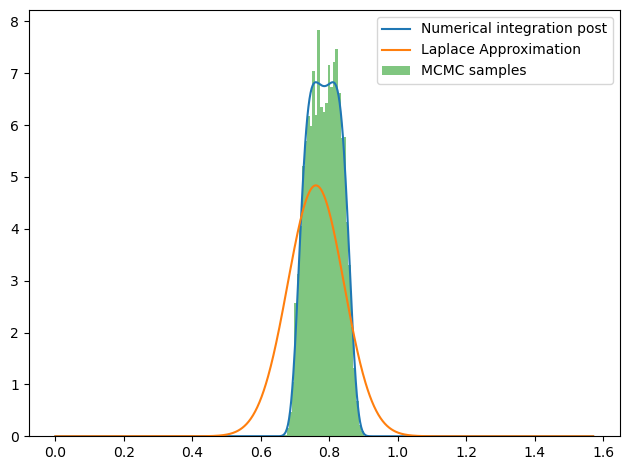
\includegraphics[width=0.7\textwidth]{laplace_MCMC_true.png}
    \caption{Laplace approximation and MCMC samples (part (e)) and the true posterior using numerical integration for the normalizing constant.}  
\end{figure}


So clearly the double peaks messes with the approximation.  
This happens in two ways. 
Firstly the ideal mean should be in the middle of the peaks, not at either one.
Secondly the hessian as an approximation for the curvature is bad, because at either one
of the peaks the curvature is less intense towards the other peak. 
Thus yielding a appoximation which is not centered well or shap enough.


\item[(g)] Using this prior, find the posterior probability that $\theta = \theta_0$, given the data.
Should Dionysus believe Artemis' claim?


prior:
\[
\theta \sim \frac{1}{2} \text{Uniform}(0, \pi/2) + \delta_{\theta_0}, \quad \theta_0 = \frac{\pi}{4} + 0.05
\]

\textbf{Solution:}
\par
Here I found two ways of doing this. Either using the given metropolis hastings algorithm. 
Using my implementation that involves passing degen=True to the function, and counting using
$== \theta_0$. 

For the other way let $H0$ be the event that $\theta = \theta_0$ and $H1$ be the event that $\theta \neq \theta_0$, but is elsewhere
on the uniform prior
\begin{align*}
    \pi(\theta = \theta_0 | x) &= \frac{\pi(x | H0) \pi(H0)}{\pi(x | H0) \pi(H0) + \pi(x | H1) \pi(H1)}\\
    &= \frac{\pi(x | H0) 1/2}{\pi(x | H0) 1/2 + \pi(x | H1) 1/2}\\
    &= \frac{\pi(x | H0)}{\pi(x | H0) + \pi(x | H1)}
    &= \frac{L(\theta_0)}{\theta_0 + \int_0^{\pi/2} L(\theta) \cdot \text{prior} d\theta}
    &= \frac{L(\theta_0)}{\theta_0 + \int_0^{\pi/2} L(\theta)  \frac{2}{\pi} d\theta}
\end{align*}

\begin{minted}{python3}
    def p_H0_num_integration(start, end):
    #integrate likelihood from start to end
    prior = 1/(end - start)
    lik_theta0 = likelihood(theta_0)
    lik_theta = quad(likelihood, start, end)[0]*prior
    return lik_theta0/(lik_theta + lik_theta0)
\end{minted}

And using numerical integration for the integral over the likelihood, I factorized out the prior, and multiplied it with it after in the code.
This gave a probability of $0.905$. So Dionysus should believe Artemis' claim.


\item[(h)] In the analysis above, the first prior component Uniform$(0, \pi/2)$ is is perhaps
a bit too broad. Therefore, repeat part (g), but with the prior

\[
\theta \sim \frac{1}{2} \text{Uniform} (\theta_0 - 0.1, \theta + 0.1) + \frac{1}{2} \delta_{\theta_0}
\]

\textbf{Solution:}
\par
Here I did the exact same as for the previous part, passing different start and end arguments
to the metropolis hastings function, and numerical integration. The probability was $0.594$. So the wider prior
was a lot better. With this prior Dionysus should maybe not believe Artemis' claim.
\end{enumerate}
    

\section{Problem 3}


\end{document}
